\chapter{Security-constrained optimal power flow (\scopflow)}\label{chap:scopflow}
SCOPFLOW solves a contingency-constrained optimal power flow problem. The problem is set up as a two-stage optimization problem where the first-stage (base-case) represents the normal operation of the grid and the second-stage comprises $N_c$ contingency scenarios. Each contingency scenario can be single or multi-period.

\section{Formulation}

\subsection{Single-period}

The contingency-constrained optimal power flow (popularly termed as security-constrained optimal power flow (SCOPF) in power system parlance) attempts to find a least cost dispatch for the base case (or no contingency) while ensuring that if any of contingencies do occur then the system will be secure. This is illustrated in Fig. \ref{fig:scopflow} for a SCOPF with a base-case $c_0$ and three contingencies.

\definecolor{lavander}{cmyk}{0,0.48,0,0}
\definecolor{violet}{cmyk}{0.79,0.88,0,0}
\definecolor{burntorange}{cmyk}{0,0.52,1,0}

\def\lav{lavander!90}
\def\oran{orange!30}

\tikzstyle{contingency}=[draw,circle,violet,bottom color=\lav,
                  top color= white, text=violet,minimum width=20pt]
\tikzstyle{base}=[draw,circle,burntorange, left color=\oran,
                       text=violet,minimum width=20pt]
                       
\tikzstyle{cedge}=[color=red]

\begin{figure}[h!]
\centering
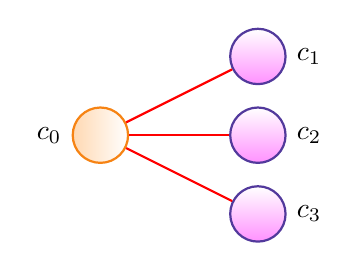
\begin{tikzpicture}[auto, thick]
  % Place base case
  \node[base,label=left:$c_0$] (base) at (0,0) {};
  
  \node[contingency,label=right:$c_1$] (c1) at (2,1) {};
  \node[contingency,label=right:$c_2$] (c2) at (2,0) {};
  \node[contingency,label=right:$c_3$] (c3) at (2,-1) {};
  
  \path[cedge] (base) edge (c1);
  \path[cedge] (base) edge (c2);
  \path[cedge] (base) edge (c3);
  
  
  
%  \foreach \place/\name in {{(0,-1)/a}, {(2,0)/b}, {(2,2)/c}, {(0,2)/d},
%           {(-2,0)/e}}
%    \node[superpeers] (\name) at \place {a};
%  \foreach \source/\dest in {a/b, a/c, a/d, b/c, c/d,a/e,d/e}
%    \path (\source) edge (\dest);
   %
   % Place normal peers
%  \foreach \pos/\i in {above left of/1, left of/2, below left of/3}
%    \node[peers, \pos = e] (e\i) {};
%   \foreach \speer/\peer in {e/e1,e/e2,e/e3}
%    \path (\speer) edge (\peer);
   %
%   \foreach \pos/\i in {above right of/1, right of/2, below right of/3}
%    \node[peers, \pos =b ] (b\i) {};
%   \foreach \speer/\peer in {b/b1,b/b2,b/b3}
%   \path (\speer) edge (\peer);
   %
%   \node[peers, above of=d] (d1){};
%   \path (d) edge (d1);
   %
%   \foreach \pos/\i in {below left of/1, below of/2}
%   \node[peers, \pos =a ] (a\i) {};
%   \foreach \speer/\peer in {a/a1,a/a2}
%   \path (\speer) edge (\peer);

\end{tikzpicture}
\caption{Contingency constrained optimal power flow example with three contingencies. $c_0$ represents the base case (or no contingency case). $c_1$, $c_2$, $c_3$ are the three contingency cases. Each of the contingency states is coupled with the base-case through ramping constraints (denoted by \textcolor{red}{red} lines)}
\label{fig:scopflow}
\end{figure}


In general form, the equations for contingency-constrained optimal power flow are given by
(\ref{eq:scopflow_start}) -- (\ref{eq:scopflow_end}). This is a two-stage stochastic optimization problem where the first stage is the base case $c_0$ and each of the contingency states $c_i, i \in [1,N_c-1]$ are second-stage subproblems. SCOPFLOW aims to minimize the objective $\sum_{c=0}^{N_c-1}f(x_c)$, while adhering to the equality $g(x_c)$, inequality $h(x_c)$, and the lower/upper bound ($x^-$,$x^+$) constraints. Equation (\ref{eq:scopflow_end}) represents the coupling between the base-case and each of the contingency states $c_i$. Equation (\ref{eq:scopflow_end}) is the most typical form of coupling that limits the deviation of the contingency variables $x_c$ from the base $x_0$ to within $\delta_c{x}$. An example of this constraint could be the allowed real power output deviation for the generators constrained by their ramp limit.


\begin{align}
\centering
\text{min}&~f(x_0)&  \label{eq:scopflow_start}\\
&\text{s.t.}& \nonumber \\
&~g(x_c) = 0,                             &c \in \left[0,N_c-1\right]& \\
&~h(x_c) \le 0,                           &c \in \left[0,N_c-1\right]& \\
x^- & \le x_c \le x^+,                     &c\in \left[0,N_c-1\right]& \\
-\delta_c{x} & \le x_c - x_0 \le \delta_c{x},&c \in \left[1,N_c\right]&
\label{eq:scopflow_end}
\end{align}

\subsection{Multiperiod}

In the multi-period version,each contingency is comprised of multiple time-periods. The multiple periods have variables and constraints as described in chapter \ref{chap:tcopflow}. An example of multi-contingency multi-period optimal power flow is illustrated in Fig. \ref{fig:ctopflow} with two contingencies $c_0$ and $c_1$. Here, $c_0$ is the case with no contingencies, i.e., the base-case. Each contingency is multi-period with four time-periods. Each time-step is coupled with its adjacent one through ramping constraints. We assume that the contingency is incident at the first time-step, i.e. at $t_0$. This results in the coupling between the contingency cases $c_i, i \in [1,N_c-1]$ and the base-case $c_0$ only at time-step $t_0$ as shown in Fig. \ref{fig:ctopflow}.

\definecolor{lavander}{cmyk}{0,0.48,0,0}
\definecolor{violet}{cmyk}{0.79,0.88,0,0}
\definecolor{burntorange}{cmyk}{0,0.52,1,0}

\def\lav{lavander!90}
\def\oran{orange!30}

\tikzstyle{time}=[draw,circle,violet,bottom color=\lav,
                  top color= white, text=violet,minimum width=20pt]
                  
\tikzstyle{base}=[draw,circle,burntorange, left color=\oran,
                       text=violet,minimum width=20pt]

\begin{figure}[h!]
\centering
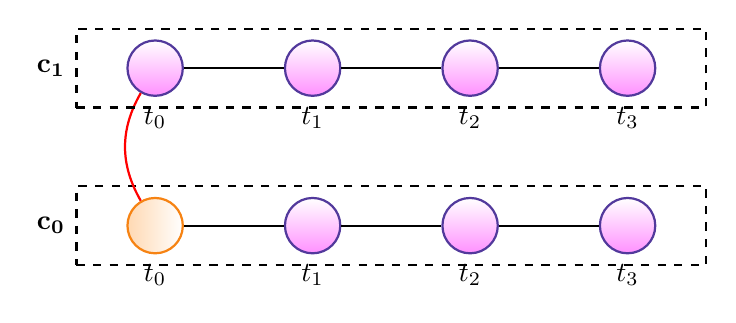
\begin{tikzpicture}[auto, thick]
  \node[base,label=below:$t_0$] (c0t0) at (0,0) {};
  \node[time,label=below:$t_1$] (c0t1) at (2,0) {};
  \node[time,label=below:$t_2$] (c0t2) at (4,0) {};
  \node[time,label=below:$t_3$] (c0t3) at (6,0) {};
  
  \path (c0t0) edge (c0t1);
  \path (c0t1) edge (c0t2);
  \path (c0t2) edge (c0t3);
  
  % rectangle from (-1.0,-0.5) to (7.0,0.5)
   \node[draw,rectangle,dashed,minimum width=8cm,minimum height=1cm,label=left:{$\mathbf{c_0}$}] (s0) at (3.0,0.0) {};
  
  \node[time,label=below:$t_0$] (c1t0) at (0,2) {};
  \node[time,label=below:$t_1$] (c1t1) at (2,2) {};
  \node[time,label=below:$t_2$] (c1t2) at (4,2) {};
  \node[time,label=below:$t_3$] (c1t3) at (6,2) {};
  
  \path (c1t0) edge (c1t1);
  \path (c1t1) edge (c1t2);
  \path (c1t2) edge (c1t3);
  
  \path (c0t0) edge [bend left,color=red] (c1t0);
  
   % rectangle from (-1.0,1.5) to (7.0,2.5)
   \node[draw,rectangle,dashed,minimum width=8cm,minimum height=1cm,label=left:{$\mathbf{c_1}$}] (s0) at (3.0,2.0) {};
  
  
  
%  \foreach \place/\name in {{(0,-1)/a}, {(2,0)/b}, {(2,2)/c}, {(0,2)/d},
%           {(-2,0)/e}}
%    \node[superpeers] (\name) at \place {a};
%  \foreach \source/\dest in {a/b, a/c, a/d, b/c, c/d,a/e,d/e}
%    \path (\source) edge (\dest);
   %
   % Place normal peers
%  \foreach \pos/\i in {above left of/1, left of/2, below left of/3}
%    \node[peers, \pos = e] (e\i) {};
%   \foreach \speer/\peer in {e/e1,e/e2,e/e3}
%    \path (\speer) edge (\peer);
   %
%   \foreach \pos/\i in {above right of/1, right of/2, below right of/3}
%    \node[peers, \pos =b ] (b\i) {};
%   \foreach \speer/\peer in {b/b1,b/b2,b/b3}
%   \path (\speer) edge (\peer);
   %
%   \node[peers, above of=d] (d1){};
%   \path (d) edge (d1);
   %
%   \foreach \pos/\i in {below left of/1, below of/2}
%   \node[peers, \pos =a ] (a\i) {};
%   \foreach \speer/\peer in {a/a1,a/a2}
%   \path (\speer) edge (\peer);

\end{tikzpicture}
\caption{Multi-period contingency constrained optimal power flow example with two contingencies $c_0$ and $c_1$, each with four time-periods $t_0$, $t_1$, $t_2$, $t_3$. State $c_0,t_0$ represent the base case (no contingency) case. We assume that any contingency is incident at the first time-step, i.e., at $t_0$. The contingency states $c_1,t_0$ is coupled with the no-contingency state $c_0,t_0$ at time $t_0$. The {\textcolor{red}{red}} line denotes the coupling between the contingency.}
\label{fig:ctopflow}
\end{figure}

The overall objective of this contingency-constrained multi-period optimal power flow is to find a secure dispatch for base-case $c_0$ while adhering to contingency and temporal constraints. The general formulation of this problem is given in Eqs. (\ref{eq:ctopflow_start}) -- (\ref{eq:ctopflow_end}).

\begin{align}
\centering
\text{min}&~\sum_{c=0}^{N_c-1}\sum_{t=0}^{N_t-1}f(x_{c,t})& \label{eq:ctopflow_start}\\
&\text{s.t.}& \nonumber \\
&~g(x_{c,t}) = 0,                                        &c \in \left[0,N_c-1\right], t \in \left[0,N_t-1\right]& \\
&~h(x_{c,t}) \le 0,                                      &c \in \left[0,N_c-1\right], t \in \left[0,N_t-1\right]& \\
x^- & \le x_{c,t} \le x^+,                               &c \in \left[0,N_c-1\right], t\in \left[0,N_t-1\right]& \\
-\delta_t{x} & \le x_{c,t} - x_{c,t-\Delta{t}} \le \delta_t{x},&c \in \left[0,N_c-1\right], t \in \left[1,N_t-1\right]& \label{eq:ctopflow_time_coupling}\\
-\delta_c{x} & \le x_{c,0} - x_{0,0} \le \delta_c{x},&c \in \left[1,N_c-1\right]& \\
\label{eq:ctopflow_end}
\end{align}

In this formulation, the objective is to reduce the cost for the base-case time horizon, where $f(x_{0,t})$ is the objective cost for contingency $c_0$ at time $t$. Equation (\ref{eq:ctopflow_end}) represents the coupling between the base case $c_0$ and each contingency $c_i$ at time-step $t_0$. We use a simple box constraint $\delta_c{x}$ to restrict the  deviation of decision variables $x_{c,0}$ from the base-case $x_{0,0}$. The bound $\delta_c{x}$ could represent here, for example, the allowable reserve for each generator.

\section{Solvers}
\scopflow can be solved with \ipopt. If one wants to solve each contingency independently, i.e., without any coupling constraints then use  the \emph{EMPAR} solver. \emph{EMPAR} distributes the contingencies to different processes when executed in parallel.

\section{Input and Output}
To execute SCOPFLOW, the following files are required:
\begin{itemize}
    \item \textbf{Network file:} The network file describing the network details. Only \matpower format files are currently supported.
    \item \textbf{Contingency file:} The file describing the contingencies. Contingencies can be single or multiple outages. The contingency file needs to be described in PTI format.
\end{itemize}
If the multi-period option is chosen, then additional files describing the load and wind generation can be (optionally) set.
\begin{itemize}
    \item \textbf{Load data:} One file for load real power and one for reactive power. The files need to be in CSV format. An example of the format for the 9-bus case is \href{https://gitlab.pnnl.gov/exasgd/frameworks/exago/-/tree/master/datafiles/case9}{here}.
    \item \textbf{Wind generation:} The wind generation time-series described in CSV format. See an example of the format \href{https://gitlab.pnnl.gov/exasgd/frameworks/exago/-/tree/master/datafiles/case9}{here}.
\end{itemize}

The \scopflow output is saved to a directory named \emph{scopflowout}. This directory contains $N_c$ files to save the solution for each contingency in MATPOWER datafile format. Each file has the name \emph{cont\_xx} where \emph{xx} is the contingency number. 

If the multi-period option is chosen then $N_c$ subdirectories are created (one for each contingency), and each subdirectory contains $N_t$ output files, one for each time-period. The subdirectories have the naming convention \emph{cont\_xx} and the output file are named as \emph{t\_yy} where \emph{yy} is the time-step number.

\section{Usage}

\begin{lstlisting}
  ./scopflow -netfile <netfilename> -ctgcfile <ctgcfilename> \
  <scopflowoptions> [-scopflow_enable_multiperiod 1]
\end{lstlisting}

\section{Options}
See table \ref{tab:scopflow_options}. In addition, all \opflow options in Table \ref{tab:opflow_options} and \tcopflow options in Table \ref{tab:tcopflow_options} can be used.
\begin{table}[!htbp]
  \caption{SCOPFLOW options}
  \small
  \begin{tabular}{|p{0.4\textwidth}|p{0.3\textwidth}|p{0.3\textwidth}|}
    \hline
    \textbf{Option} & \textbf{Meaning} & \textbf{Values (Default value)} \\ \hline
    -netfile & Network file name & string $<$ 4096 characters (\href{https://gitlab.pnnl.gov/exasgd/frameworks/exago/-/blob/master/datafiles/case9/case9mod_gen3_wind.m}{case9mod\_gen3\_wind.m}) \\ \hline
    -ctgcfile & Contingency file name & string $<$ 4096 characters (\href{https://gitlab.pnnl.gov/exasgd/frameworks/exago/-/blob/master/datafiles/case9/case9.cont}{case9.cont}) \\ \hline
    -save\_output & Save output to directory & 0 or 1 (0) \\ \hline
    -scopflow\_solver & Set solver for scopflow & IPOPT or EMPAR \\ \hline
    -scopflow\_Nc & Number of contingencies & int (0. Passing -1 results in all contingencies in the file used) \\ \hline
    -scopflow\_mode & Operation mode: Preventive or corrective & 0 or 1 (0) \\ \hline
    -scopflow\_iscoupling & Coupling between first and second stage & 0 or 1 (0) \\ \hline
    -scopflow\_enable\_multiperiod & Multi-period SCOPFLOW & 0 or 1 (0) \\ \hline \hline
    -scopflow\_pload\_profile & Real power load profile & string (\href{https://gitlab.pnnl.gov/exasgd/frameworks/exago/-/blob/master/datafiles/case9/load_P.csv}{load\_P.csv}) \\ \hline
    -scopflow\_qload\_profile & Reactive power load profile & string (\href{https://gitlab.pnnl.gov/exasgd/frameworks/exago/-/blob/master/datafiles/case9/load_Q.csv}{load\_Q.csv}) \\ \hline
    -scopflow\_windgenprofile & Wind generation profile & string (\href{https://gitlab.pnnl.gov/exasgd/frameworks/exago/-/blob/master/datafiles/case9/scenarios_9bus.csv}{case9/scenarios\_9bus.csv}) \\ \hline
    -scopflow\_dT & Length of time-step (minutes) & double (5.0) \\ \hline
    -scopflow\_duration & Total duration (hours) & double (0.5) \\ \hline 
  \end{tabular}
  \label{tab:scopflow_options}
\end{table}

Depending on the \emph{mode}, SCOPFLOW can either be \emph{preventive} (mode = 0) or \emph{corrective} (mode = 1). In the preventive mode, the PV and PQ generator real power is fixed to its corresponding base-case values. The generators at the reference bus pick up any make-up power required for the contingency. The corrective mode allows deviation of the PV and PQ generator real power from the base-case dispatch constrained by its 30-min. ramp rate capability.

-scopflow\_enable\_multiperiod 1 must be used in order to enable any of the options listed in table \ref{tab:scopflow_options} that are below -scopflow\_enable\_multiperiod.

\section{Examples}

Some \scopflow example runs are provided with some sample output. Options are the default options given in table \ref{tab:opflow_options}, \ref{tab:tcopflow_options} and \ref{tab:scopflow_options} unless otherwise specified. Sample output is generated by running examples in the installation directory.

Example using the \ipopt solver:

\begin{lstlisting}
$ ./bin/scopflow -scopflow_solver IPOPT -tcopflow_iscoupling 1 \
-scopflow_iscoupling 1 -print_output
[ExaGO INFO]: -- Checking ... -options_file not passed        exists: no
SCOPFLOW: Application created
SCOPFLOW running with 2 contingencies (base case + 1 contingencies)
Rank 0 has 2 contingencies, range [0 -- 2]
SCOPFLOW: Using IPOPT solver
SCOPFLOW: Setup completed

*************************************************************************
This program contains Ipopt, a library for large-scale nonlinear 
optimization. Ipopt is released as open source code under the Eclipse 
Public License (EPL).
*************************************************************************

This is Ipopt version 3.12.10, running with linear solver ma27.

Number of nonzeros in equality constraint Jacobian...:      231
Number of nonzeros in inequality constraint Jacobian.:      182
Number of nonzeros in Lagrangian Hessian.............:      249

Total number of variables............................:       55
                     variables with only lower bounds:        0
                variables with lower and upper bounds:       39
                     variables with only upper bounds:        0
Total number of equality constraints.................:       44
Total number of inequality constraints...............:       59
        inequality constraints with only lower bounds:       21
   inequality constraints with lower and upper bounds:       38
        inequality constraints with only upper bounds:        0

iter  objective  inf_pr  inf_du lg(mu) ||d|| lg(rg) alpha_du alpha_pr  ls
0  7.4421250e+03 1.80e+00 1.69e+01  -1.0 0.00e+00 - 0.00e+00 0.00e+00   0
1  6.9108233e+03 1.65e+00 1.56e+01  -1.0 1.24e+00 - 4.46e-02 8.38e-02f  1
2  5.9991119e+03 1.30e+00 5.10e+01  -1.0 7.41e-01 - 7.07e-02 2.08e-01f  1
...
43 3.0556401e+03 1.07e-14 3.95e-10  -8.6 2.79e-09 - 1.00e+00 1.00e+00f  1

Number of Iterations....: 43

                                   (scaled)                 (unscaled)
Objective...........:   6.8512110967619464e+01    3.0556401491558281e+03
Dual infeasibility..:   3.9453703519053556e-10    1.7596351769497887e-08
Constraint violation:   1.0658141036401503e-14    1.0658141036401503e-14
Complementarity.....:   5.0027986112663857e-09    2.2312481806248081e-07
Overall NLP error...:   5.0027986112663857e-09    2.2312481806248081e-07


Number of objective function evaluations             = 59
Number of objective gradient evaluations             = 44
Number of equality constraint evaluations            = 59
Number of inequality constraint evaluations          = 59
Number of equality constraint Jacobian evaluations   = 44
Number of inequality constraint Jacobian evaluations = 44
Number of Lagrangian Hessian evaluations             = 43
Total CPU secs in IPOPT (w/o function evaluations)   =      0.019
Total CPU secs in NLP function evaluations           =      0.009

EXIT: Optimal Solution Found.
=============================================================
        Security-Constrained Optimal Power Flow
=============================================================
OPFLOW Formulation                  POWER_BALANCE_POLAR
Solver                              IPOPT
Initialization                      MIDPOINT
Number of contingencies             1
Load loss allowed                   NO
Power imbalance allowed             NO
Ignore line flow constraints        NO

Number of variables                 57
Number of equality constraints      42
Number of inequality constraints    58
Number of coupling constraints      3

Convergence status                  CONVERGED
Objective value                     3055.64

----------------------------------------------------------------------
Bus        Pd      Qd      Vm      Va      mult_Pmis      mult_Qmis
----------------------------------------------------------------------
1         0.00    0.00   1.040   0.000      2158.80        -0.00
2         0.00    0.00   1.025   4.572      2108.44         0.00
3         0.00    0.00   1.025   1.912      2118.81         0.00
4         0.00    0.00   1.038  -2.306      2159.07        -0.61
5        75.00   30.00   1.026  -3.550      2170.87         2.93
6        90.00   30.00   1.023  -4.551      2191.34         4.30
7         0.00    0.00   1.033   0.613      2109.20         4.12
8       100.00   35.00   1.022  -2.070      2133.92         7.92
9         0.00    0.00   1.036  -0.462      2119.23         2.84

-------------------------------------------------------------------------
From       To       Status     Sft      Stf     Slim     mult_Sf  mult_St
-------------------------------------------------------------------------
1          4          1       75.61    75.44   380.00    -0.00    -0.00
2          7          1      117.34   118.26   250.00    -0.00    -0.00
3          9          1       76.90    77.68   300.00    -0.00    -0.00
4          5          1       28.64    34.88   250.00    -0.00    -0.00
4          6          1       46.84    48.91   250.00    -0.00    -0.00
5          7          1       47.56    50.96   250.00    -0.00    -0.00
6          9          1       45.96    48.57   150.00    -0.00    -0.00
7          8          1       69.77    70.78   250.00    -0.00    -0.00
8          9          1       37.09    30.76   150.00    -0.00    -0.00

-------------------------------------------------------------------------
Gen   Status  Fuel     Pg       Qg       Pmin     Pmax     Qmin     Qmax
-------------------------------------------------------------------------
1       1     COAL    75.40     5.62    10.00   350.00  -300.00   300.00
2       1     COAL   116.97    -9.31    10.00   300.00  -300.00   300.00
3       1     WIND    75.00   -16.97     0.00    75.00  -300.00   300.00
[ExaGO INFO]: Finalizing scopflow application
\end{lstlisting}

Example using the IPOPT solver with multiperiod enabled:

\begin{lstlisting}
$./bin/scopflow -scopflow_solver IPOPT -scopflow_enable_multiperiod 1 \
-tcopflow_iscoupling 1 -scopflow_iscoupling 1
[ExaGO INFO]: -- Checking ... -options_file not passed         exists: no
SCOPFLOW: Application created
SCOPFLOW running with 2 contingencies (base case + 1 contingencies)
Rank 0 has 2 contingencies, range [0 -- 2]
SCOPFLOW: Using IPOPT solver
TCOPFLOW: Application created
TCOPFLOW: Duration = 0.166667 hours, timestep = 5.000000 minutes, \
          number of time-steps = 3
TCOPFLOW: Using IPOPT solver
TCOPFLOW: Setup completed
TCOPFLOW: Application created
TCOPFLOW: Duration = 0.166667 hours, timestep = 5.000000 minutes, \
          number of time-steps = 3
TCOPFLOW: Using IPOPT solver
TCOPFLOW: Setup completed
SCOPFLOW: Setup completed

*************************************************************************
This program contains Ipopt, a library for large-scale nonlinear 
optimization. Ipopt is released as open source code under the 
Eclipse Public License (EPL).
*************************************************************************

This is Ipopt version 3.12.10, running with linear solver ma27.

Number of nonzeros in equality constraint Jacobian...:      640
Number of nonzeros in inequality constraint Jacobian.:      494
Number of nonzeros in Lagrangian Hessian.............:      540

Total number of variables............................:      138
                     variables with only lower bounds:        0
                variables with lower and upper bounds:       90
                     variables with only upper bounds:        0
Total number of equality constraints.................:      110
Total number of inequality constraints...............:      151
        inequality constraints with only lower bounds:       36
   inequality constraints with lower and upper bounds:      115
        inequality constraints with only upper bounds:        0

iter objective inf_pr  inf_du lg(mu)  ||d||  lg(rg) alpha_du alpha_pr  ls
0  4.4652750e+04 1.80e+00 5.01e+01 -1.0 0.00e+00 - 0.00e+00 0.00e+00   0
1  3.1127309e+04 1.41e+00 1.01e+02 -1.0 1.97e+00 - 1.87e-01 2.18e-01f  1
...
55  1.7423413e+04 9.91e-15 8.48e-10 -8.6 9.66e-09 - 1.00e+00 1.00e+00h  1

Number of Iterations....: 55

                                   (scaled)                 (unscaled)
Objective...........:   3.9065947675497836e+02    1.7423412663272036e+04
Dual infeasibility..:   8.4833681960093011e-10    3.7835822154201486e-08
Constraint violation:   9.9087404947795221e-15    9.9087404947795221e-15
Complementarity.....:   3.3875752035319637e-09    1.5108585407752560e-07
Overall NLP error...:   3.3875752035319637e-09    1.5108585407752560e-07


Number of objective function evaluations             = 91
Number of objective gradient evaluations             = 56
Number of equality constraint evaluations            = 91
Number of inequality constraint evaluations          = 91
Number of equality constraint Jacobian evaluations   = 56
Number of inequality constraint Jacobian evaluations = 56
Number of Lagrangian Hessian evaluations             = 55
Total CPU secs in IPOPT (w/o function evaluations)   =      0.045
Total CPU secs in NLP function evaluations           =      0.052

EXIT: Optimal Solution Found.
[ExaGO INFO]: Finalizing scopflow application.
\end{lstlisting}

Example using the \emph{EMPAR} solver with multiperiod enabled:

\begin{lstlisting}
$ ./bin/scopflow -scopflow_solver EMPAR -scopflow_enable_multiperiod 1 \
-tcopflow_iscoupling 1 -scopflow_iscoupling 1
[ExaGO INFO]: -- Checking ... -options_file not passed       exists: no
SCOPFLOW: Application created
SCOPFLOW running with 2 contingencies (base case + 1 contingencies)
Rank 0 has 2 contingencies, range [0 -- 2]
SCOPFLOW: Using EMPAR solver
TCOPFLOW: Application created
TCOPFLOW: Duration = 0.166667 hours, timestep = 5.000000 minutes, 
          number of time-steps = 3
TCOPFLOW: Using IPOPT solver
TCOPFLOW: Setup completed
TCOPFLOW: Application created
TCOPFLOW: Duration = 0.166667 hours, timestep = 5.000000 minutes, 
          number of time-steps = 3
TCOPFLOW: Using IPOPT solver
TCOPFLOW: Setup completed
SCOPFLOW: Setup completed
Setting: "0" is not a valid setting for Option: tol. 
Check the option documentation.

### tol (Real Number) ###
Category: Convergence
Description: Desired convergence tolerance (relative).
0 < (1e-08) <= +inf

********************************************************************
This program contains Ipopt, a library for large-scale nonlinear 
optimization. Ipopt is released as open source code under 
the Eclipse Public License (EPL).
********************************************************************

This is Ipopt version 3.12.10, running with linear solver ma27.

Number of nonzeros in equality constraint Jacobian...:      330
Number of nonzeros in inequality constraint Jacobian.:      258
Number of nonzeros in Lagrangian Hessian.............:      270

Total number of variables............................:       69
                     variables with only lower bounds:        0
                variables with lower and upper bounds:       45
                     variables with only upper bounds:        0
Total number of equality constraints.................:       54
Total number of inequality constraints...............:       78
        inequality constraints with only lower bounds:       18
   inequality constraints with lower and upper bounds:       60
        inequality constraints with only upper bounds:        0

iter  objective  inf_pr  inf_du lg(mu) ||d|| lg(rg) alpha_du alpha_pr  ls
0  2.2326375e+04 1.80e+00 5.02e+01  -1.0 0.00e+00 - 0.00e+00 0.00e+00   0
1  1.5533385e+04 1.40e+00 1.02e+02  -1.0 1.95e+00 - 1.88e-01 2.20e-01f  1
...
32  8.6735595e+03 7.99e-15 3.70e-09  -8.6 1.93e-08 - 1.00e+00 1.00e+00h 1

Number of Iterations....: 32

                                   (scaled)                 (unscaled)
Objective...........:   1.9447442817603635e+02    8.6735594966512217e+03
Dual infeasibility..:   3.6983296779767669e-09    1.6494550363776382e-07
Constraint violation:   7.9936057773011271e-15    7.9936057773011271e-15
Complementarity.....:   4.9913149587308981e-09    2.2261264715939807e-07
Overall NLP error...:   4.9913149587308981e-09    2.2261264715939807e-07


Number of objective function evaluations             = 40
Number of objective gradient evaluations             = 33
Number of equality constraint evaluations            = 40
Number of inequality constraint evaluations          = 40
Number of equality constraint Jacobian evaluations   = 33
Number of inequality constraint Jacobian evaluations = 33
Number of Lagrangian Hessian evaluations             = 32
Total CPU secs in IPOPT (w/o function evaluations)   =      0.019
Total CPU secs in NLP function evaluations           =      0.014

EXIT: Optimal Solution Found.
Setting: "0" is not a valid setting for Option: tol. 
Check the option documentation.

### tol (Real Number) ###
Category: Convergence
Description: Desired convergence tolerance (relative).
0 < (1e-08) <= +inf
This is Ipopt version 3.12.10, running with linear solver ma27.

Number of nonzeros in equality constraint Jacobian...:      306
Number of nonzeros in inequality constraint Jacobian.:      234
Number of nonzeros in Lagrangian Hessian.............:      270

Total number of variables............................:       69
                     variables with only lower bounds:        0
                variables with lower and upper bounds:       45
                     variables with only upper bounds:        0
Total number of equality constraints.................:       54
Total number of inequality constraints...............:       72
        inequality constraints with only lower bounds:       18
   inequality constraints with lower and upper bounds:       54
        inequality constraints with only upper bounds:        0

iter objective  inf_pr   inf_du lg(mu) ||d|| lg(rg) alpha_du alpha_pr  ls
0  2.2326375e+04 1.80e+00 4.89e+01  -1.0 0.00e+00 - 0.00e+00 0.00e+00   0
1  1.5535979e+04 1.41e+00 1.01e+02  -1.0 1.97e+00 - 1.87e-01 2.18e-01f  1
...
51  8.7491131e+03 8.88e-15 4.80e-09  -8.6 1.07e-08 - 1.00e+00 1.00e+00h  1

Number of Iterations....: 51

                                (scaled)               (unscaled)
Objective...........:   1.9616845456090007e+02    8.7491130734161434e+03
Dual infeasibility..:   4.8019002633480731e-09    2.1416475174532407e-07
Constraint violation:   8.8817841970012523e-15    8.8817841970012523e-15
Complementarity.....:   4.9761717933322852e-09    2.2193726198261992e-07
Overall NLP error...:   4.9761717933322852e-09    2.2193726198261992e-07


Number of objective function evaluations             = 54
Number of objective gradient evaluations             = 52
Number of equality constraint evaluations            = 54
Number of inequality constraint evaluations          = 54
Number of equality constraint Jacobian evaluations   = 52
Number of inequality constraint Jacobian evaluations = 52
Number of Lagrangian Hessian evaluations             = 51
Total CPU secs in IPOPT (w/o function evaluations)   =      0.024
Total CPU secs in NLP function evaluations           =      0.016

EXIT: Optimal Solution Found.
[ExaGO INFO]: Finalizing scopflow application.
\end{lstlisting}
